
\usepackage{hyperref}

%\usetheme{vub}
\usetheme[coloredtitles]{vub}
%\usetheme[showsection]{vub}

\title{Knowledge transfer in deep reinforcement learning}
% \subtitle{Master thesis}
\author{Arno Moonens}
\date{June 30, 2017}

% To center the contents of a frame vertically
\makeatletter
\define@key{beamerframe}{c}[true]{% centered
  \beamer@frametopskip=0pt plus 1fill\relax%
  \beamer@framebottomskip=0pt plus 1fill\relax%
  \beamer@frametopskipautobreak=0pt plus .4\paperheight\relax%
  \beamer@framebottomskipautobreak=0pt plus .6\paperheight\relax%
  \def\beamer@initfirstlineunskip{}%
}
\makeatother

% To change footnote size
\let\oldfootnotesize\footnotesize
\renewcommand*{\footnotesize}{\oldfootnotesize\tiny}

\setbeamertemplate{caption}{\raggedright\insertcaption\par}

\AtBeginPart{\frame{\partpage}}
% \AtBeginSection{\frame{\sectionpage}}
% \AtBeginSubsection{\frame{\subsectionpage}}

\graphicspath{ {../images/} }

\makeatletter
\def\beamer@framenotesbegin{% at beginning of slide
  \gdef\beamer@noteitems{}%
  \gdef\beamer@notes{{}}% used to be totally empty.
}
\makeatother

\begin{document}
\frame{\titlepage}

\begin{frame}{Outline}
    \vskip0pt plus 3fill
  {\color{vubbleu}\large Background}
  \tableofcontents[part=1]

  {\color{vubbleu}\large Experiments}
  \tableofcontents[part=2]

  {\color{vubbleu}\large Conclusions}
  \tableofcontents[part=3]
\end{frame}

\part{Background}

\section{Artificial neural networks}
\begin{frame}[fragile]\frametitle{Artificial neural networks}
% \framesubtitle{Architecture}
\vskip0pt plus 3fill
\begin{columns}
\begin{column}{0.5\textwidth}
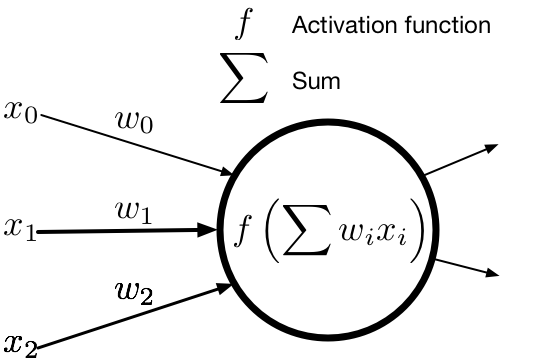
\includegraphics[width=\linewidth]{neuron.png}
\end{column}
\vrule
\begin{column}{0.5\textwidth}
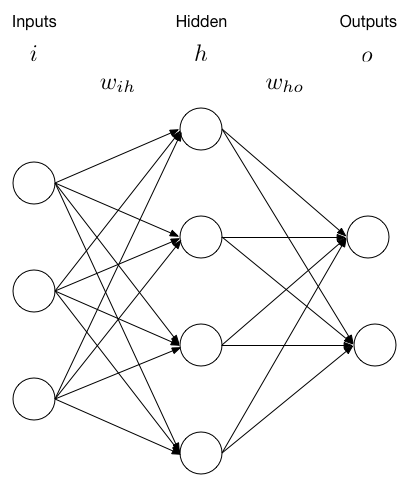
\includegraphics[width=\linewidth]{ann.png}
\end{column}
\end{columns}
\note{
    \begin{itemize}
        \item ANN = function approximator
        \item multiple layers each with units
        \item each unit: non-linear function of linear combination of units at previous layer
        \item each connection between units can vary in strength
        \item Error is differentiated to compute change in weights (backpropagation)
    \end{itemize}
}
\end{frame}

\section{Deep learning}
\begin{frame}[t]\frametitle{Deep learning}
\framesubtitle{Convolutional neural networks}
\vskip0pt plus 0.9fill
\begin{center}
    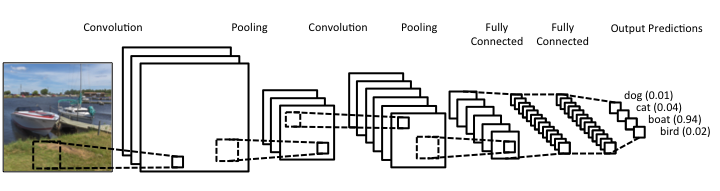
\includegraphics[width=\linewidth]{cnnlayout.png} \footnote{Source: \cite{clarifai}}\\
    \vskip0pt plus 0.1fill
    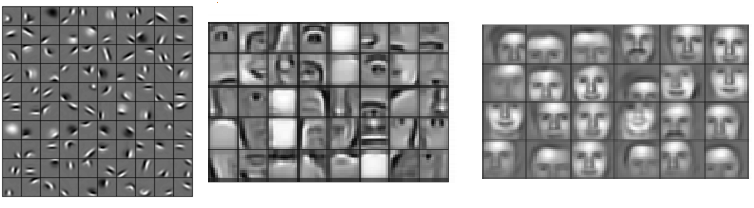
\includegraphics[width=\linewidth]{cnnfeatures.png} \footnote{Source: \cite{conf/icml/LeeGRN09}}
\end{center}
\note{
\begin{itemize}
    \item Handle high-dimensional data
    \item CNN = primarily used for images
    \item Slide filter over image
    \item Each level higher level representations
\end{itemize}
}
\end{frame}

\section{Reinforcement learning}
\begin{frame}[fragile]\frametitle{Reinforcement learning}
\vskip0pt plus 1fill
\begin{center}
    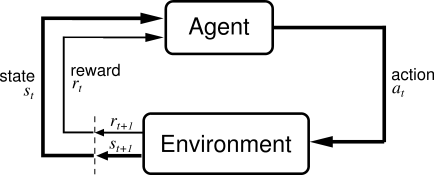
\includegraphics[width=.7\linewidth]{reinforcementlearning.png}
    \footnote{Source: \url{https://www.analyticsvidhya.com/blog/2017/01/introduction-to-reinforcement-learning-implementation/}}
\end{center}
\begin{itemize}
    \item Goal: maximize total reward
    \begin{itemize}
        \item By changing its policy $\pi$
    \end{itemize}
    \item Policy gradient:
    \begin{itemize}
        \item Policy is parametrized: $\pi_\theta(s,a)$
        \item Input: states
        \item Output: action (probabilities)
    \end{itemize}
\end{itemize}
\note{
    \begin{itemize}
        \item Learn by trial-and-error
        \item Use policy to select actions
        \item Action produced using value function for state and action or directly: policy gradient
        \item Policy gradient:
        \begin{itemize}
            \item Parameterized policy
            \item Action probabilities
            \item Parameters updated to improve rewards
        \end{itemize}
    \end{itemize}
}
\end{frame}

\section{Deep reinforcement learning}
\begin{frame}[fragile]{Deep reinforcement learning}
\framesubtitle{A3C architecture}
\vskip0pt plus 10fill
\begin{center}
    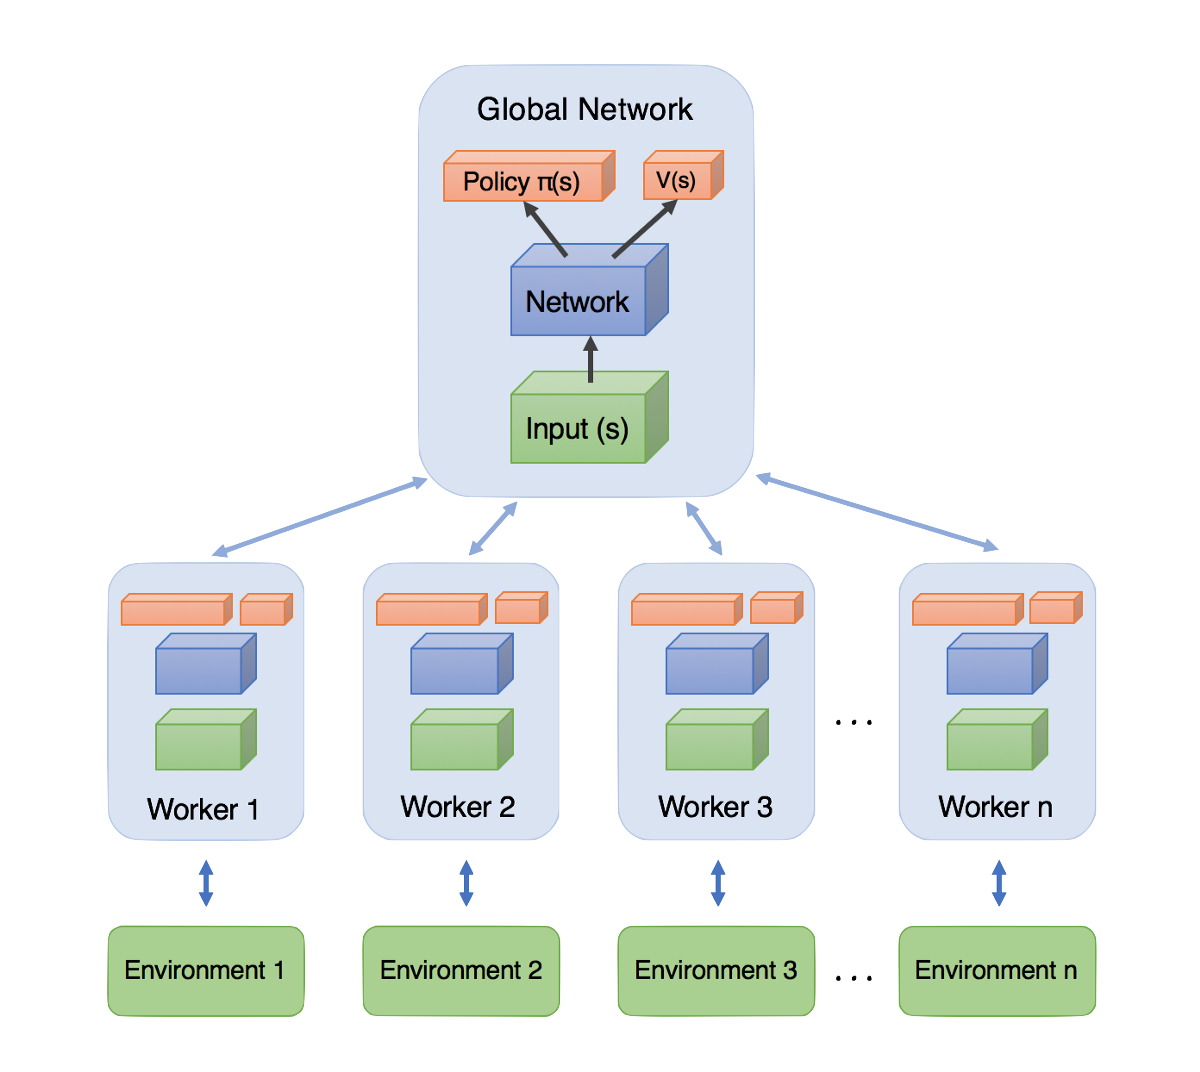
\includegraphics[width=.7\linewidth]{A3Carchitecture} \footnote{Source: \cite{Juliani2016A3C}}
\end{center}
\note{
    \begin{itemize}
        \item Combination of deep learning \& reinforcement learning
        \item Applied on environments with images as input
        \item Able to deal with correlated subsequent observations (they cause instability)
        \item A3C
        \begin{itemize}
            \item Learn in parallel on same kind of environment (same parameters)
            \item Global network with all the weights
            \item Each worker has copy
            \item Worker learns and then updates weights of global network
        \end{itemize}
    \end{itemize}
}
\end{frame}

\section{Transfer learning}
\begin{frame}[fragile]{Transfer learning}
\vskip0pt plus 1fill
\begin{columns}
\begin{column}{0.4\textwidth}
\begin{itemize}
    \item Which knowledge?
    \item From which tasks?
    \item How are tasks related?
    \begin{itemize}
        \item Same state space?
        \item Same action space?
    \end{itemize}
    \item Which RL algorithms are allowed?
\end{itemize}
\end{column}
    \begin{column}{0.6\textwidth}
    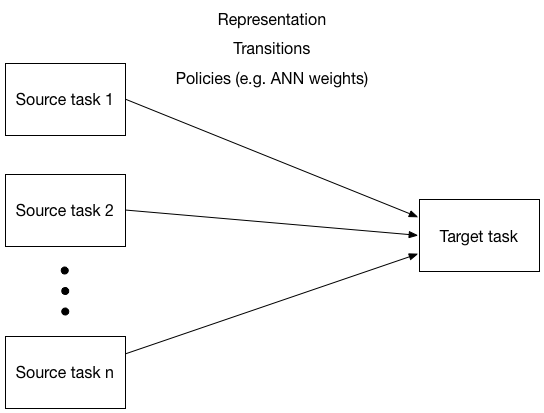
\includegraphics[width=\linewidth]{transfer_learning}
    \end{column}
\end{columns}
\begin{center}
\end{center}
\note{
    \begin{itemize}
        \item Use information about source task to improve target task performance
        \begin{itemize}
            \item Jumpstart, Asymptotic, Total reward, Time until threshold
        \end{itemize}
        \item Transfer representation (FE), transitions or policies
        \item Tasks with same/different state and action space
        \begin{itemize}
            \item Task mapping may be necessary
        \end{itemize}
    \end{itemize}
}
\end{frame}

\part{Experiments}
\section{Proposed algorithm}
\begin{frame}[fragile]{Proposed algorithm}
\framesubtitle{Architecture}
\vskip0pt plus 1fill
\begin{center}
    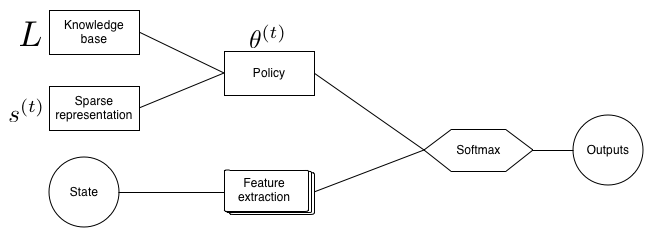
\includegraphics[width=\linewidth]{knowledge_transfer.png}
\end{center}
\note{
    \begin{itemize}
        \item Policy factorized as knowledge base \& sparse representation
        \begin{itemize}
            \item Shared knowledge base
            \item Shared feature extraction
            \item Each task has own sparse representation
        \end{itemize}
        \item Softmax to get action probabilities
    \end{itemize}
}
\end{frame}

\begin{frame}[fragile]{Proposed algorithm}
\framesubtitle{Learning source tasks}
\vskip1.5cm plus 2fill
\begin{center}
    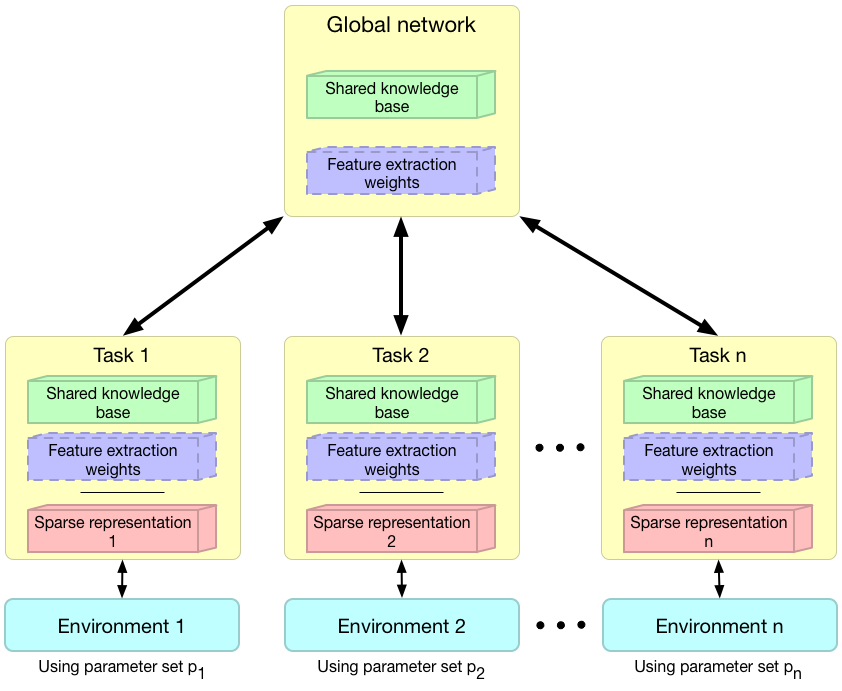
\includegraphics[width=.75\linewidth]{knowledge_transfer_tasks.png}
\end{center}
\note{
    \begin{itemize}
        \item Similar to A3C
        \item Global network has no sparse representation
        \item Each environment has different parameters (next slide)
        \item Global network is always transferred to target task
        \item Random sparse repr. can also be transferred
    \end{itemize}
}
\end{frame}

\section{Experimental setup}
\begin{frame}[fragile]{Experimental setup}
\framesubtitle{Environments}
\vskip1.1cm plus 2.5fill
\begin{figure}[htb]
    \begin{minipage}{0.55\textwidth}
            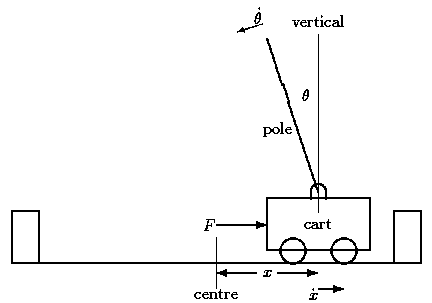
\includegraphics[width=\linewidth]{cartpole.png}
            \caption{Cart-Pole. Source: \cite{grant1990modelling}.}
            \vskip0.9cm
            \begin{itemize}
                \item Different cart mass
                \item Different pole mass \& length
            \end{itemize}
    \end{minipage}\hfill
    \begin{minipage}{0.45\textwidth}
            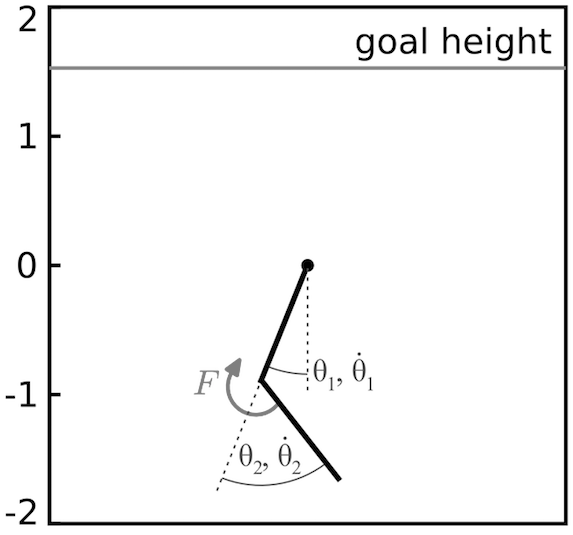
\includegraphics[width=\linewidth]{acrobot.png}
            \caption{Acrobot. Source: \cite{fremaux2013reinforcement}.}
            \begin{itemize}
                \item Different length \& mass for each pole
            \end{itemize}
    \end{minipage}
\end{figure}
\note{
    \begin{itemize}
        \item Cart-pole:
        \begin{itemize}
            \item Balance pole on cart as long as possible
            \item Force on cart
            \item Different cart mass
            \item Different pole mass \& length
        \end{itemize}
        \item Acrobot:
        \begin{itemize}
            \item 2 joint arms
            \item Outer point must be above threshold in min. steps
            \item Different arm lengths and masses
        \end{itemize}
    \end{itemize}
}
\end{frame}

\section{Results}
\frame{\sectionpage}
\begin{frame}[fragile]{Parallel and sequential knowledge transfer}
\framesubtitle{Cart-pole}
\vskip0pt plus 3fill
\begin{center}
    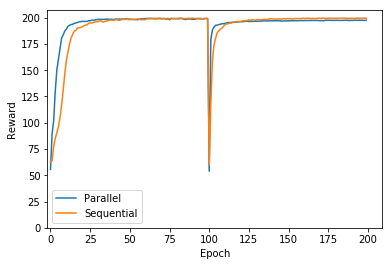
\includegraphics[width=.8\linewidth]{results/CartPole/kt_akt/reward_source-target_5tasks.png}
\end{center}
\end{frame}

\begin{frame}[fragile]{Feature extraction}
\framesubtitle{Cart-pole}
\vskip0pt plus 3fill
\begin{center}
    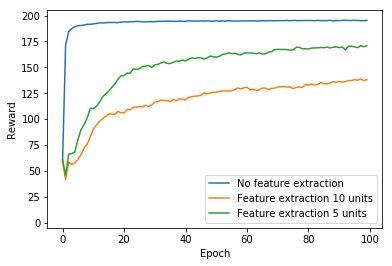
\includegraphics[width=.8\linewidth]{results/CartPole/feature_extraction.png}
\end{center}
\end{frame}

\begin{frame}[fragile]{Different amount of source tasks}
\framesubtitle{Cart-pole}
\vskip1.5cm plus 0.5cm minus 0.1cm
Using 5 and 10 tasks, compared with \textit{REINFORCE}.
\begin{center}
    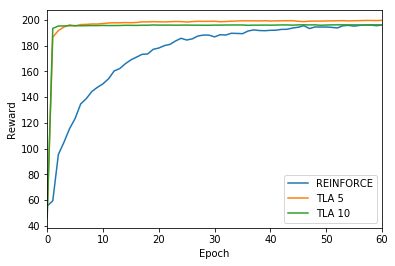
\includegraphics[width=.8\linewidth]{results/CartPole/no_sparse_transfer/reward_target_re-akt5-akt10.png}
\end{center}
\end{frame}

\begin{frame}[fragile]{Different amount of source tasks}
\framesubtitle{Acrobot}
\vskip0pt plus 3fill
\begin{center}
    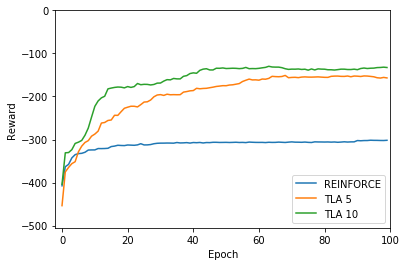
\includegraphics[width=.8\linewidth]{results/Acrobot/no_sparse_transfer/reward_target_re-akt5-akt10.png}
\end{center}
\end{frame}

\begin{frame}[fragile]{Transfer of sparse representation}
\framesubtitle{Cart-pole}
\vskip1.5cm plus 0.5cm minus 0.1cm
Transfer of shared knowledge base and randomly chosen sparse representation.
\begin{center}
    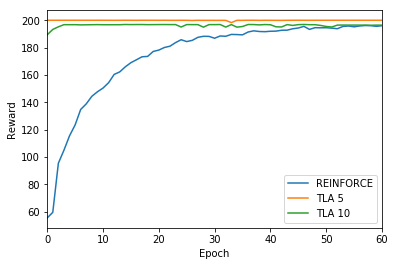
\includegraphics[width=.8\linewidth]{results/CartPole/sparse_transfer/reward_target_re-akt5-akt10.png}
\end{center}
\end{frame}

\begin{frame}[fragile]{Transfer of sparse representation}
\framesubtitle{Acrobot}
\vskip0pt plus 3fill
\begin{center}
    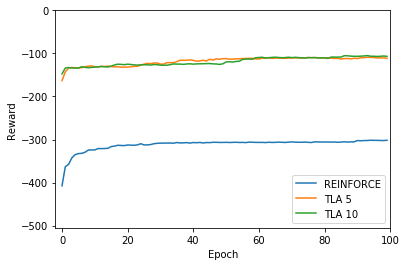
\includegraphics[width=.8\linewidth]{results/Acrobot/sparse_transfer/reward_target_re-akt5-akt10.png}
\end{center}
\end{frame}

\begin{frame}[fragile]{REINFORCE using a source and target task}
\framesubtitle{Cart-pole}
\vskip1.5cm plus 0.5cm minus 0.1cm
Transfer of ANN weights.
\begin{center}
    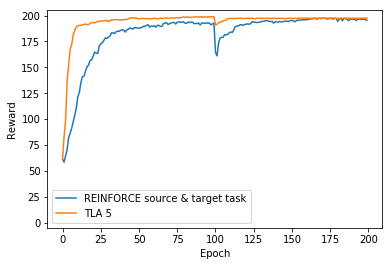
\includegraphics[width=.8\linewidth]{results/CartPole/reinforce_2tasks.png}
\end{center}
\end{frame}

\begin{frame}[fragile]{REINFORCE using a source and target task}
\framesubtitle{Acrobot}
\vskip0pt plus 3fill
\begin{center}
    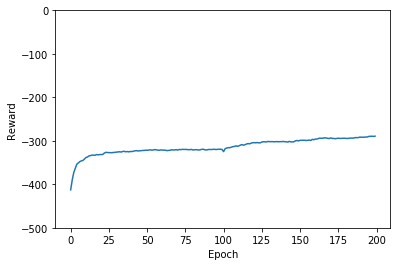
\includegraphics[width=.8\linewidth]{results/Acrobot/reinforce_2tasks.png}
\end{center}
\end{frame}

\part{Conclusions}
\section{Conclusions}
\begin{frame}[fragile]{Conclusions}
\begin{itemize}
    \item Parallel learning on source tasks better than sequentially
    \item Feature extraction wasn't beneficial for \textit{cart-pole} and \textit{acrobot}
    \item Our algorithm performs better than \textit{REINFORCE}
    \item It is better to use multiple source tasks
\end{itemize}
\end{frame}


\begin{frame}[fragile]{Conclusions}
\framesubtitle{Future work}
\begin{itemize}
    \item Apply on environments with feature extraction (e.g. \textit{Pong}, \textit{Breakout})
    \item Transfer between different environments
    \begin{itemize}
        \item Using task mappings
    \end{itemize}
\end{itemize}
\end{frame}

\begin{frame}[c]{The end}
\begin{center}
    \color{vubbleu} \LARGE\vubfont Thank you for listening!
\end{center}
\end{frame}

\begin{frame}[allowframebreaks]
\frametitle{References}
\footnotesize{
\bibliographystyle{apalike}
\bibliography{../Mendeley.bib}
}
\end{frame}

\end{document}
